\documentclass[12pt,a4paper]{article}
\usepackage[a4paper,margin=1in]{geometry}
\usepackage{graphicx}
\usepackage{amsmath}
\usepackage{hyperref}
\usepackage{setspace}
\graphicspath{{diagrams/}}
\setstretch{1.15}
\setlength{\parskip}{0.25em}
\setlength{\parindent}{0pt}

\begin{document}

\title{CloudNotes: A Cloud-Native Notes Platform with Automated Delivery, Traffic-Based Scaling, and Observability}
\author{INT378: Advancements in Cloud and DevOps\\Lovely Professional University\\Savinay Singh}
\date{}
\maketitle

\begin{abstract}
CloudNotes is a notes-management application and DevOps demonstration. It separates a web frontend, REST API, and PostgreSQL persistence service into independently deployable containers. Terraform describes AWS infrastructure, including a virtual private cloud, EC2 instances, and an S3 bucket. Jenkins is configured to test and scan the application, publish Docker images, and deploy a release to Kubernetes. Kubernetes provides service discovery, ingress routing, health-based recovery, and horizontal pod scaling. KEDA is configured to use Prometheus request-rate metrics to scale application pods. Prometheus collects backend metrics; Grafana is provisioned for the local Docker Compose environment. Repository configuration documents the intended deployment; a live cloud deployment and scaling run require separate current evidence.
\end{abstract}

\noindent\textbf{Keywords:} Cloud Computing, DevOps, Docker, Kubernetes, KEDA, Terraform, AWS, Jenkins, Prometheus, Grafana, CI/CD.

\section{Introduction}
Modern web applications must be delivered quickly while remaining available, observable, and capable of adapting to changing demand. Manual server configuration and manual deployment are error-prone because the resulting environment is difficult to reproduce and scale. CloudNotes addresses this problem by applying DevOps practices across the complete application lifecycle. The project uses version-controlled infrastructure, independently packaged services, automated build and deployment stages, and live monitoring.

CloudNotes allows users to create, read, update, search, and delete notes through a browser interface. Although the application domain is intentionally simple, its deployment architecture reflects the concerns of a production-oriented cloud service. The frontend is responsible for the user interface, the backend exposes REST endpoints and domain logic, and PostgreSQL provides durable data storage. These components communicate through defined service interfaces rather than being deployed as a single monolithic process.

Figure~\ref{fig:system_architecture} presents the system at a high level.

\begin{figure}[htbp]
\centering
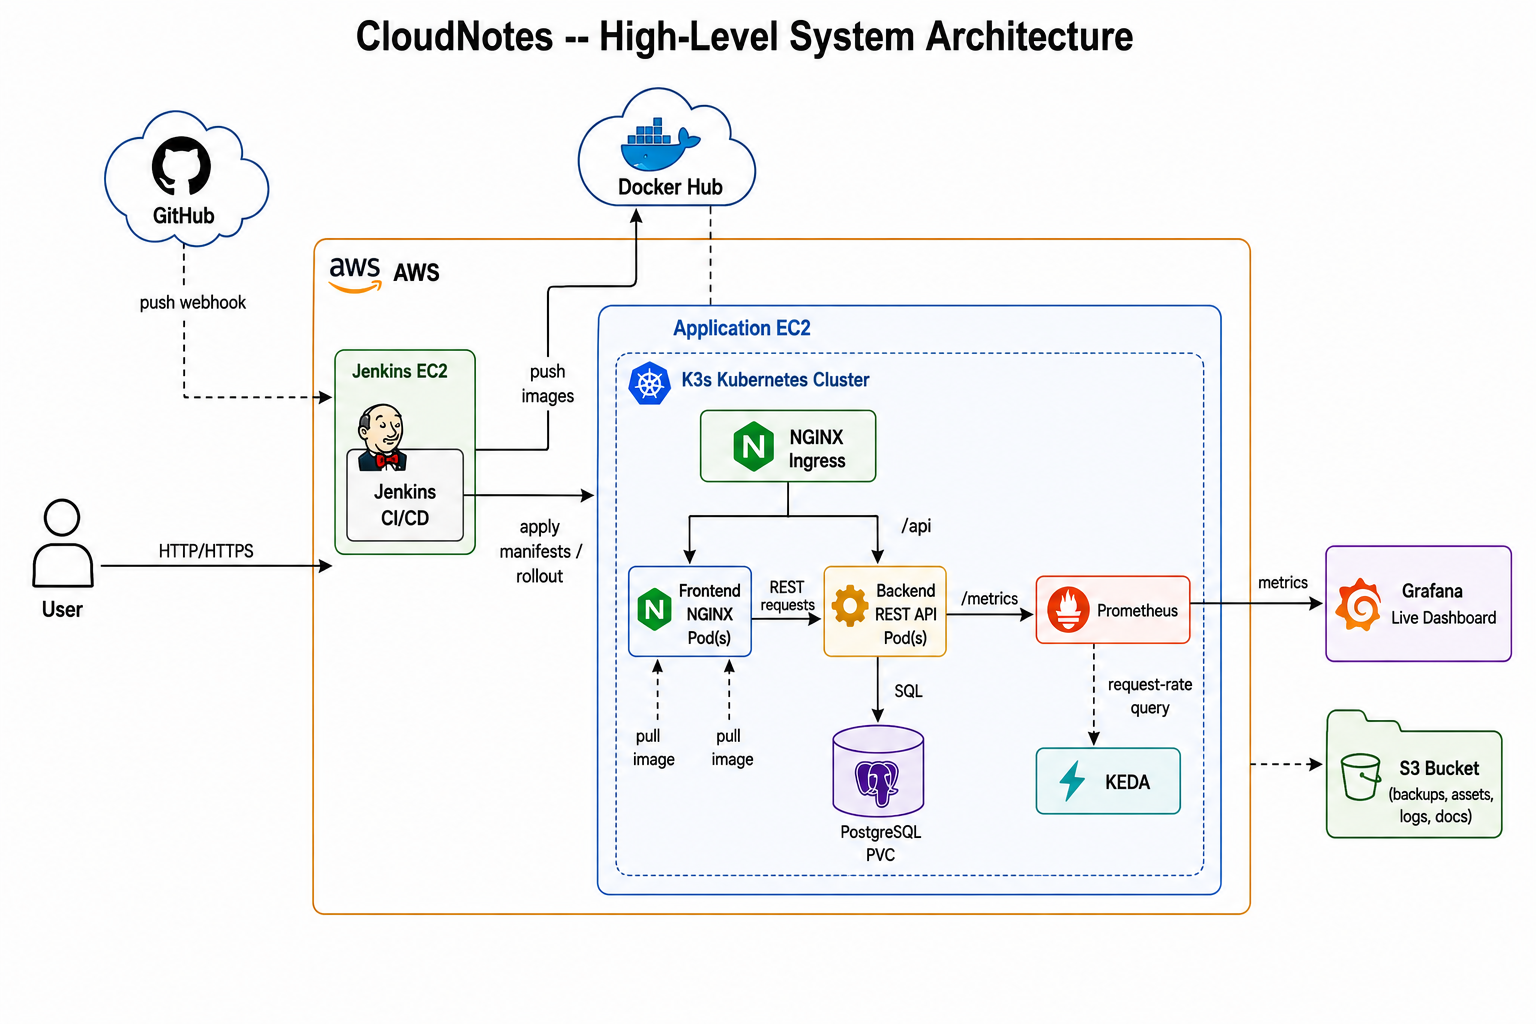
\includegraphics[width=0.82\linewidth,height=0.42\textheight,keepaspectratio]{system_architecture.png}
\caption{CloudNotes high-level system architecture}
\label{fig:system_architecture}
\end{figure}

\section{Problem Statement}
Traditional deployments often couple application code, runtime dependencies, configuration, and server setup. This coupling makes releases difficult to repeat and makes it hard to react safely to increased traffic. Teams also need visibility into application health, request volume, latency, failures, and resource behaviour in order to diagnose operational problems.

The problem addressed by this project is to design and implement a reproducible cloud deployment for a multi-service web application that supports independent service packaging, AWS infrastructure provisioning, automated delivery from source control, horizontal scaling based on traffic, and live monitoring. The solution must avoid vertical autoscaling and must not rely on GitHub Actions for the delivery pipeline.

\section{Objectives and Scope}
The primary objectives of CloudNotes are:
\begin{enumerate}
    \item Containerize the frontend and backend as independently buildable Docker images, while operating PostgreSQL as a separate service.
    \item Provision repeatable AWS infrastructure with Terraform, including EC2 compute resources and S3 object storage.
    \item Deploy the application to Kubernetes for orchestration, service discovery, ingress routing, recovery, and horizontal scaling.
    \item Scale application replicas using request-rate metrics collected by Prometheus, rather than using vertical scaling.
    \item Automate test, image build, security scan, image publication, and Kubernetes deployment stages through Jenkins and GitHub webhooks.
    \item Provide live Prometheus and Grafana observability for availability, request activity, latency, errors, memory usage, and note operations.
\end{enumerate}

The scope is limited to the CloudNotes application and its associated DevOps infrastructure. The project includes local Docker Compose support for development and a Kubernetes-oriented AWS demonstration path. It does not implement multi-region disaster recovery, enterprise identity management, or a managed database service. Sensitive values are represented as deployment-time configuration and must be replaced with secure values before any public deployment.

\subsection{Functional Requirements}
The unauthenticated demonstration application allows a user to create a note with a title and body, retrieve stored notes, search notes by text, edit an existing note, and delete a note. In containerized environments, operations are persisted in PostgreSQL. The backend exposes REST resources under the \texttt{/api/notes} path, and the frontend consumes these resources through the same browser-facing application endpoint. A dedicated \texttt{/api/health} resource supports deployment health checks, while \texttt{/metrics} exposes operational measurements.

\subsection{Non-Functional Requirements}
The design emphasizes repeatability, loose coupling, observability, and recoverability. A service must be deployable from its own image definition. Infrastructure must be expressible as Terraform configuration instead of undocumented manual setup. The deployment pipeline must detect a source-control event, test the application, identify common security risks, and report a failed rollout. The system must maintain at least two frontend and backend replicas and scale horizontally as measured traffic rises. Finally, monitoring data must be visible in a dashboard that refreshes without manual page reload.

Figure~\ref{fig:use_case} summarises the main user and operator interactions with the platform.

\begin{figure}[htbp]
\centering
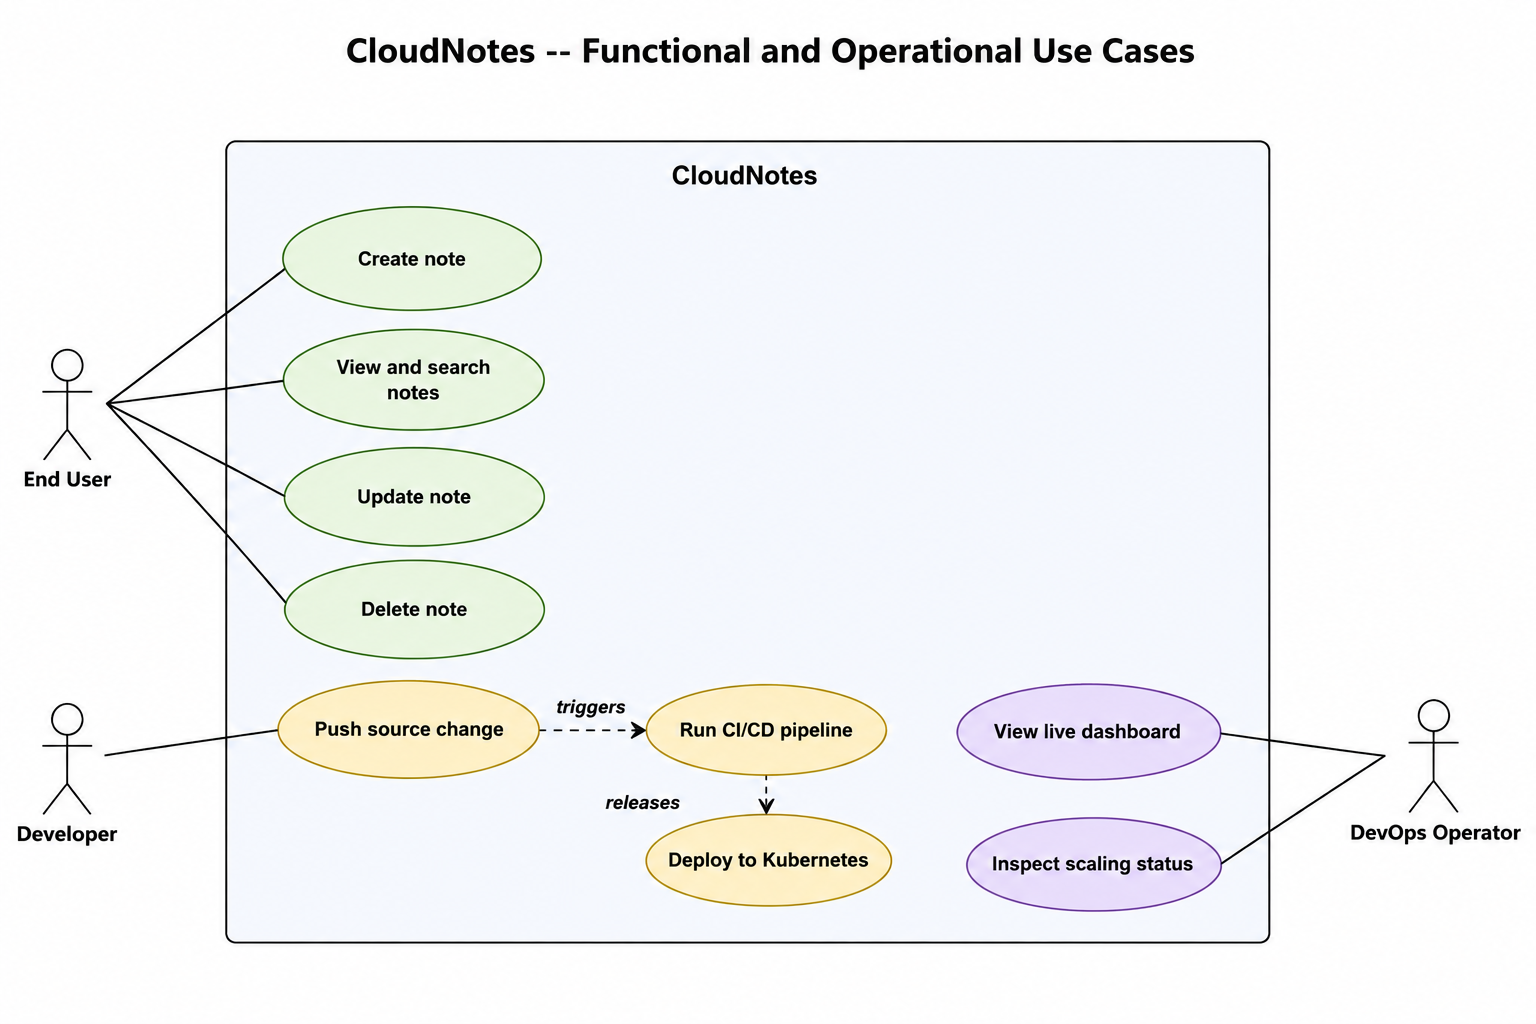
\includegraphics[width=0.82\linewidth,height=0.42\textheight,keepaspectratio]{cloudnotes_use_case.png}
\caption{CloudNotes functional and operational use cases}
\label{fig:use_case}
\end{figure}

\section{System Architecture and Containerization}
The application follows a three-tier architecture. The frontend is served by NGINX and forwards API requests to the backend service. The backend provides REST endpoints for note operations, exposes a health endpoint for readiness checks, and publishes a \texttt{/metrics} endpoint. PostgreSQL stores note records on persistent storage. Dockerfiles define the runtime environment for the frontend and backend independently, allowing either component to be rebuilt and released without recompiling the other.

For local development, Docker Compose creates a private bridge network and starts the database, frontend, backend, Prometheus, and Grafana services together. For the AWS deployment path, Kubernetes manifests define Deployments for the frontend, backend, PostgreSQL, and Prometheus services. Kubernetes Services provide stable internal names, and a PersistentVolumeClaim protects PostgreSQL data across pod recreation.

Kubernetes health probes are configured for the backend. A liveness probe enables Kubernetes to restart an unhealthy container, while a readiness probe prevents traffic from reaching the backend before it is ready. An NGINX Ingress controller routes external HTTP traffic to the frontend and backend services. Figure~\ref{fig:k8s_architecture} shows the Kubernetes deployment and request flow.

The component boundaries are intentionally explicit. The frontend never accesses PostgreSQL directly; it depends only on the backend API. Similarly, the backend does not contain ingress, dashboard, or infrastructure responsibilities. This separation reduces the impact of a change to any one tier and makes each service easier to test, package, and scale independently. Figure~\ref{fig:component_architecture} shows these responsibilities and communication interfaces.

\begin{figure}[htbp]
\centering
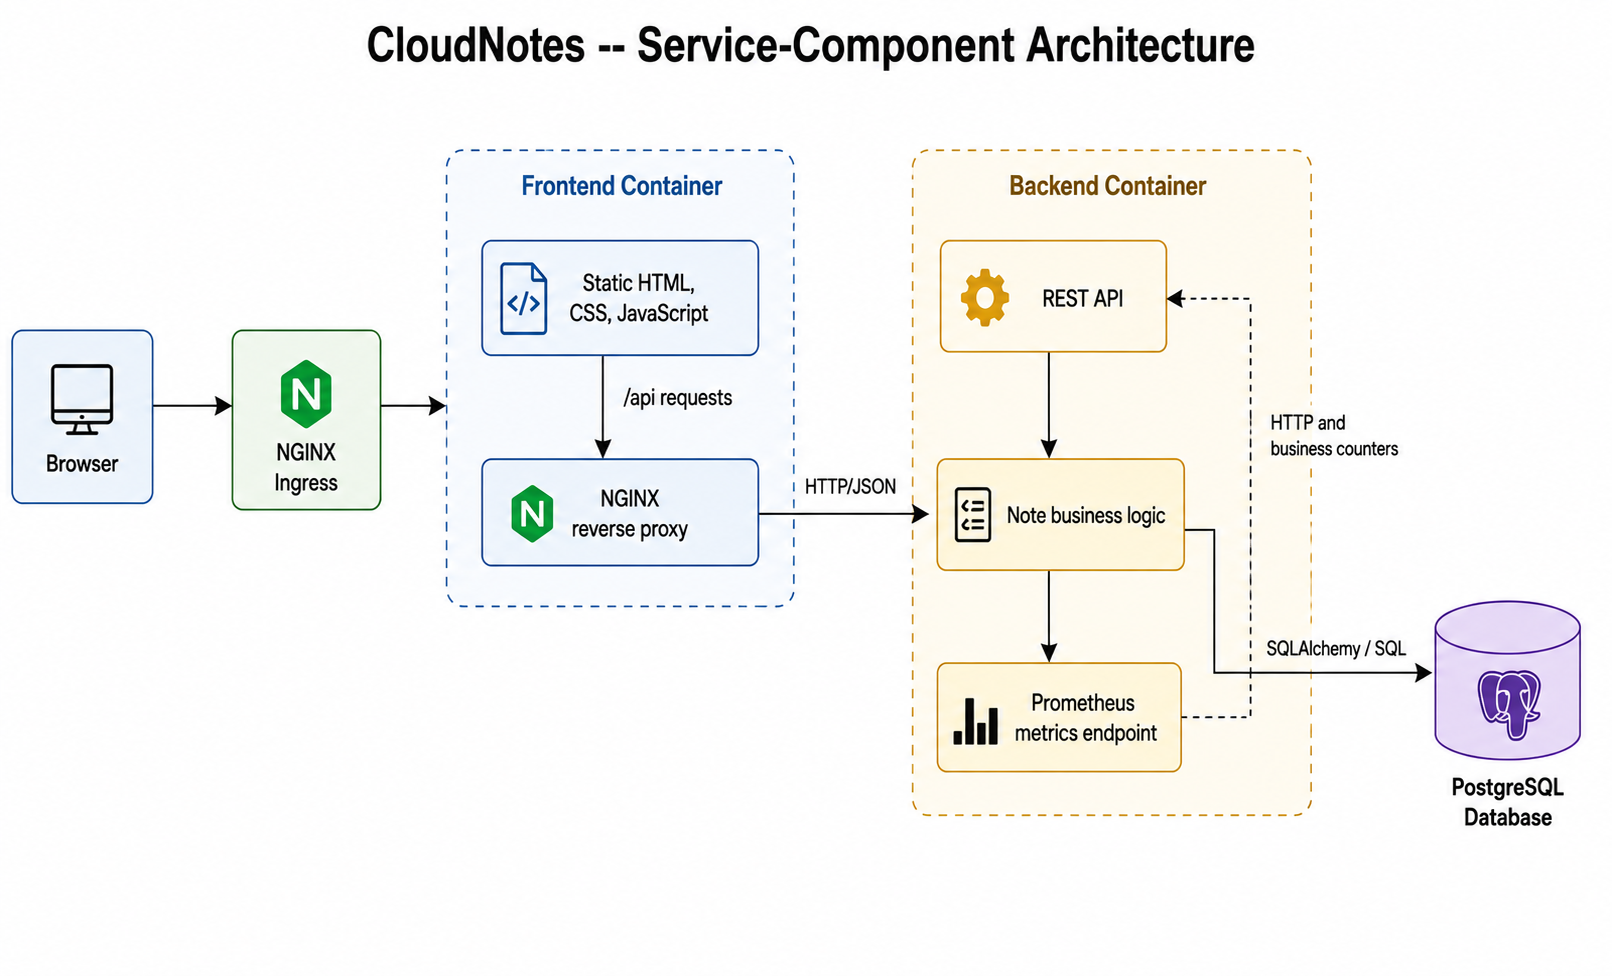
\includegraphics[width=0.82\linewidth,height=0.42\textheight,keepaspectratio]{service_component_architecture.png}
\caption{CloudNotes service-component architecture}
\label{fig:component_architecture}
\end{figure}

\begin{figure}[htbp]
\centering
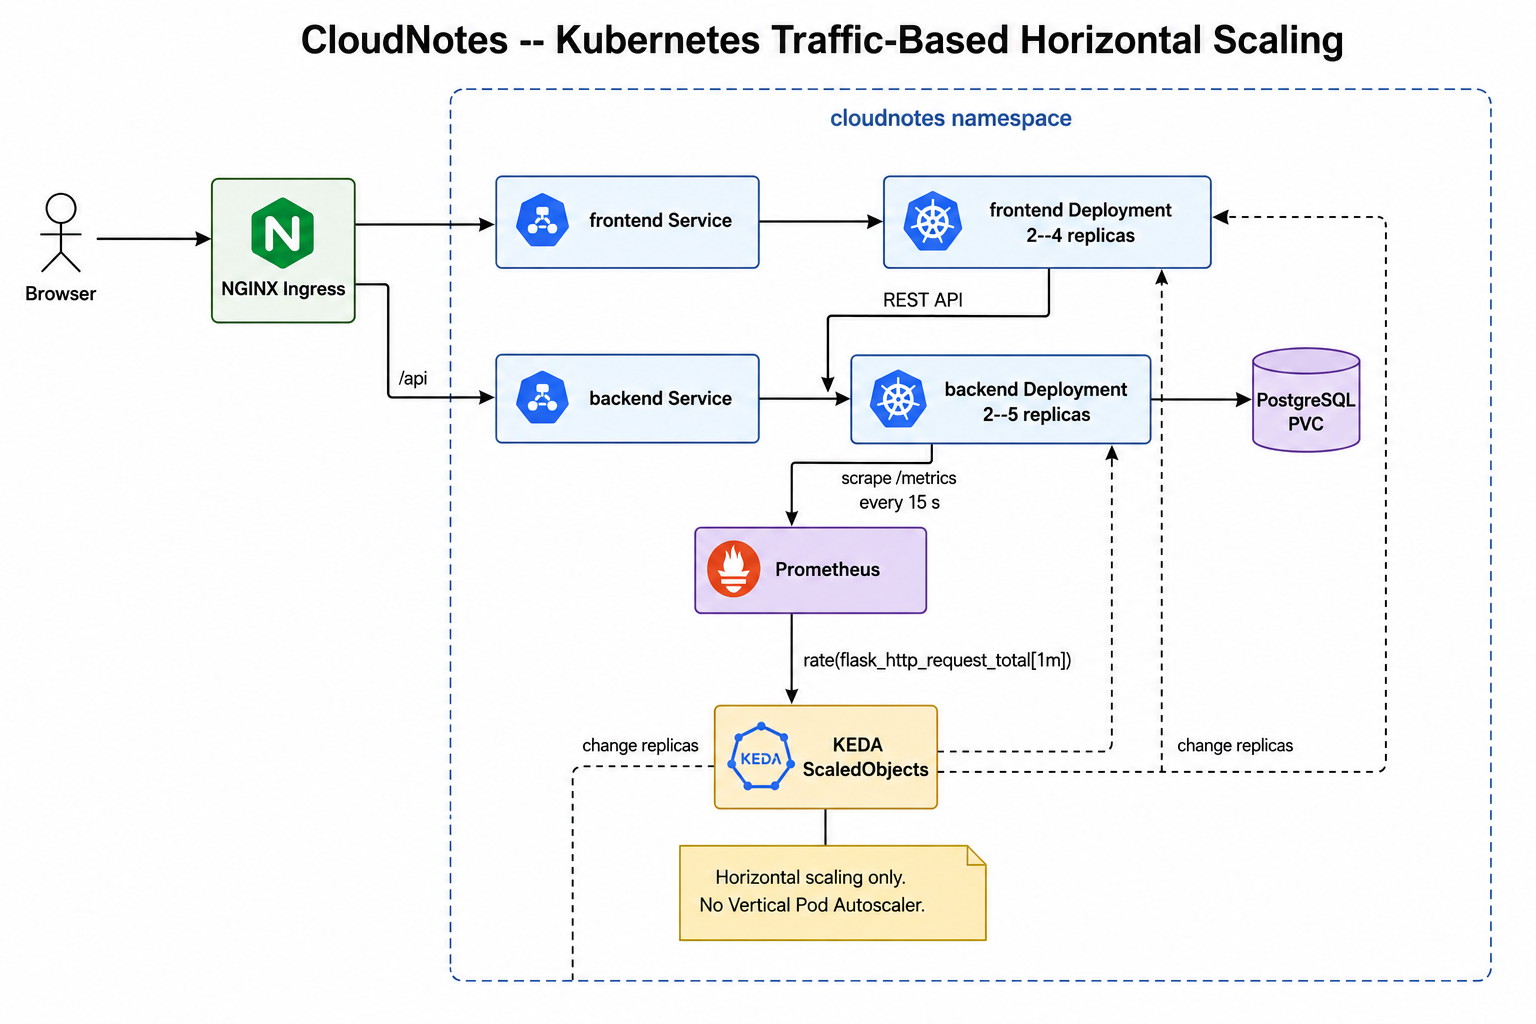
\includegraphics[width=0.82\linewidth,height=0.42\textheight,keepaspectratio]{k8s_traffic_scaling.png}
\caption{Kubernetes deployment and traffic-based horizontal scaling}
\label{fig:k8s_architecture}
\end{figure}

\section{Infrastructure Provisioning on AWS}
Terraform implements infrastructure as code for the AWS environment. Its configuration defines a VPC, public subnet, internet gateway, route table, security groups, SSH key pair, EC2 instances, and an S3 bucket. One EC2 instance hosts Jenkins, while another hosts the Kubernetes distribution used for application deployment. The application security group permits web traffic on ports 80 and 443, while SSH access is available for controlled administration.

The Terraform bootstrap configuration installs K3s, a lightweight Kubernetes distribution, on the application instance. It also installs the NGINX Ingress Controller and KEDA. KEDA integrates with Prometheus and creates the autoscaling resources needed for traffic-driven horizontal scaling. Keeping this configuration in source control makes the target environment repeatable and reviewable. Figure~\ref{fig:terraform_architecture} describes the infrastructure relationship.

\begin{figure}[htbp]
\centering
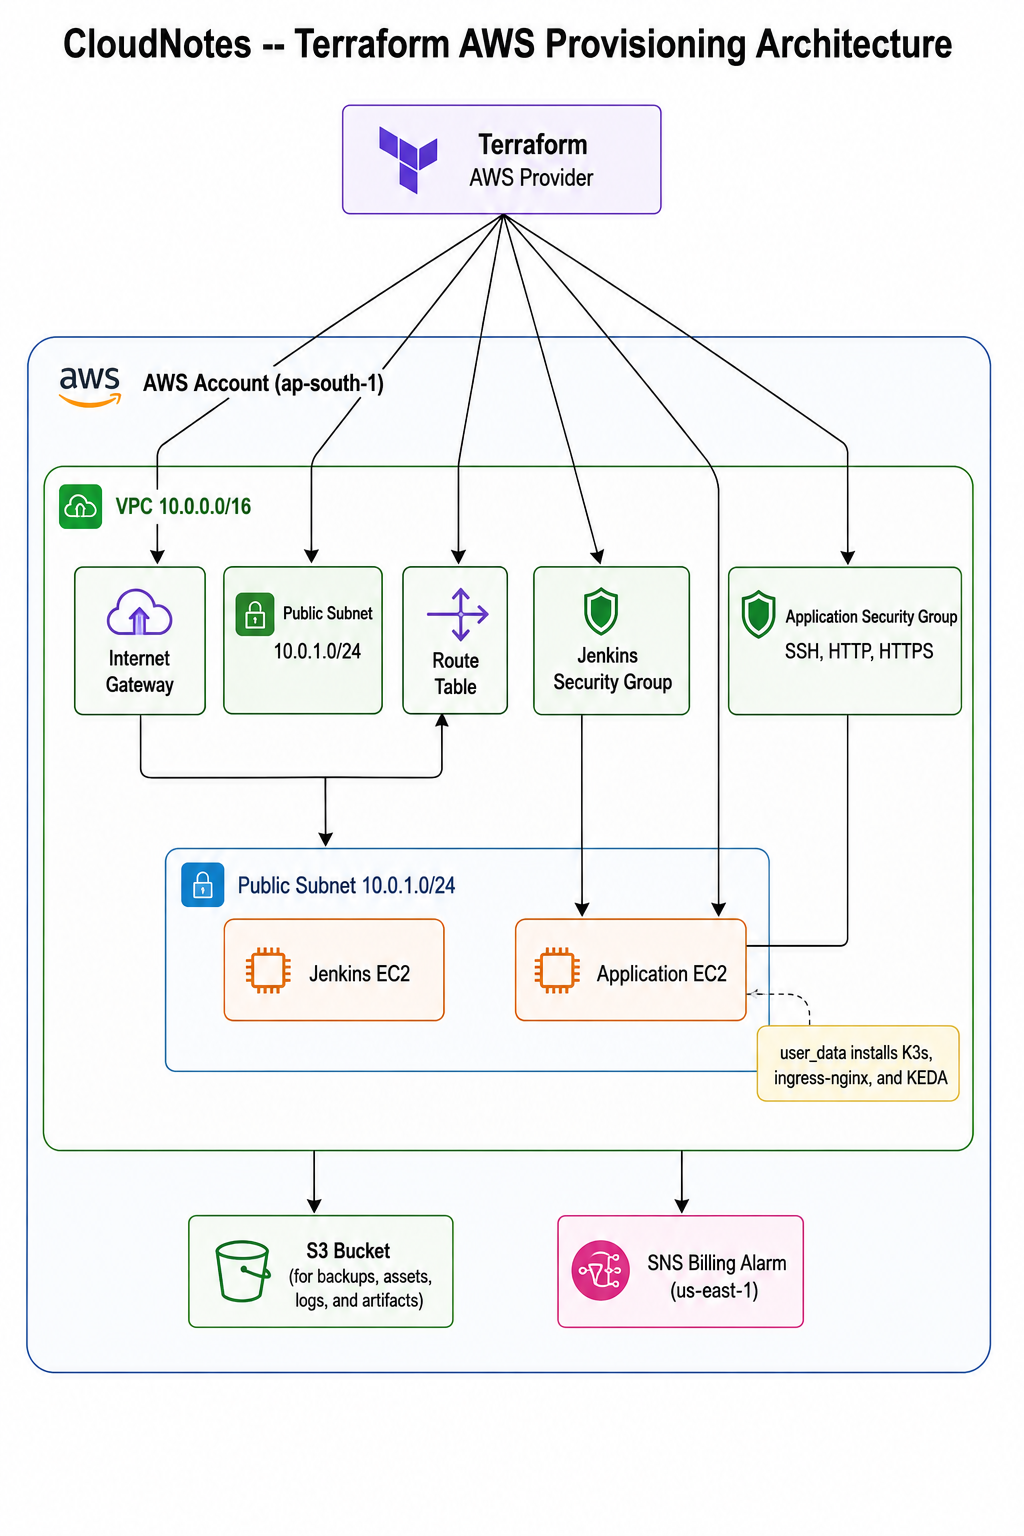
\includegraphics[width=0.72\linewidth,height=0.48\textheight,keepaspectratio]{terraform_aws_architecture.png}
\caption{Terraform-provisioned AWS infrastructure}
\label{fig:terraform_architecture}
\end{figure}

\section{Current Implementation Status}
The repository contains Dockerfiles, Kubernetes manifests, Prometheus and Grafana configuration, Terraform modules, a billing alarm, a Jenkins pipeline, and deployment automation. The current scaling manifest defines KEDA ScaledObjects that query Prometheus request-rate metrics at 15-second intervals. The Jenkinsfile describes manifest application, image updates, rollout checks, and an ingress health check. Whether these steps have succeeded in a particular environment must be confirmed from current Terraform, Jenkins, Kubernetes, Prometheus, and Grafana output; configuration files alone are not runtime evidence.

\section{Development Methodology}
CloudNotes follows an iterative DevOps methodology: implement a feature, test it in containers, commit it to GitHub, build and scan images with Jenkins, deploy versioned images, and observe the result through Prometheus and Grafana. Infrastructure, manifests, dashboard definitions, and pipeline logic remain in version control, reducing configuration drift and enabling release traceability through Jenkins build tags.

\section{Module Specification}
Table~\ref{tab:modules} describes the responsibilities and principal interfaces of the main modules. The modular design ensures that the user interface, application logic, persistence, delivery automation, infrastructure, and monitoring can evolve with minimal direct coupling.

\begin{table}[htbp]
\caption{CloudNotes module specification}
\label{tab:modules}
\centering
\begin{tabular}{p{0.18\textwidth}p{0.28\textwidth}p{0.42\textwidth}}
\hline
\textbf{Module} & \textbf{Responsibility} & \textbf{Inputs and outputs} \\
\hline
Frontend & Presents note-management user interface and forwards API requests. & Receives browser requests; sends JSON API requests to the backend; renders note data and errors. \\
Backend API & Validates requests, applies note operations, exposes health and metrics endpoints. & Receives REST requests; reads/writes PostgreSQL data; returns JSON, health status, and Prometheus metrics. \\
PostgreSQL & Provides durable relational storage for notes. & Receives SQL operations from backend only; stores note title, body, identifier, and timestamp. \\
Terraform & Defines AWS network, compute, storage, security, and bootstrap configuration. & Receives variables and AWS credentials; creates EC2, S3, VPC, security groups, and related resources. \\
Jenkins & Automates integration and deployment activities. & Receives GitHub webhook; produces test results, scan results, Docker tags, and Kubernetes rollout. \\
Kubernetes/KEDA & Runs services and adjusts replica counts from traffic metrics. & Receives manifests and images; exposes Services; produces healthy replicas and scaling events. \\
Prometheus/Grafana & Collects, analyses, and visualizes operational telemetry. & Receives \texttt{/metrics} samples; produces PromQL results, alerts, and live dashboard panels. \\
\hline
\end{tabular}
\end{table}

\section{Deployment Topology}
Jenkins runs on a dedicated EC2 instance, while the application EC2 instance hosts K3s, the ingress controller, KEDA, Prometheus, and the CloudNotes namespace. Kubernetes Services decouple callers from individual pod addresses, so pods can be recreated or scaled without changing application endpoints. Figure~\ref{fig:deployment_topology} shows these boundaries.

\begin{figure}[htbp]
\centering
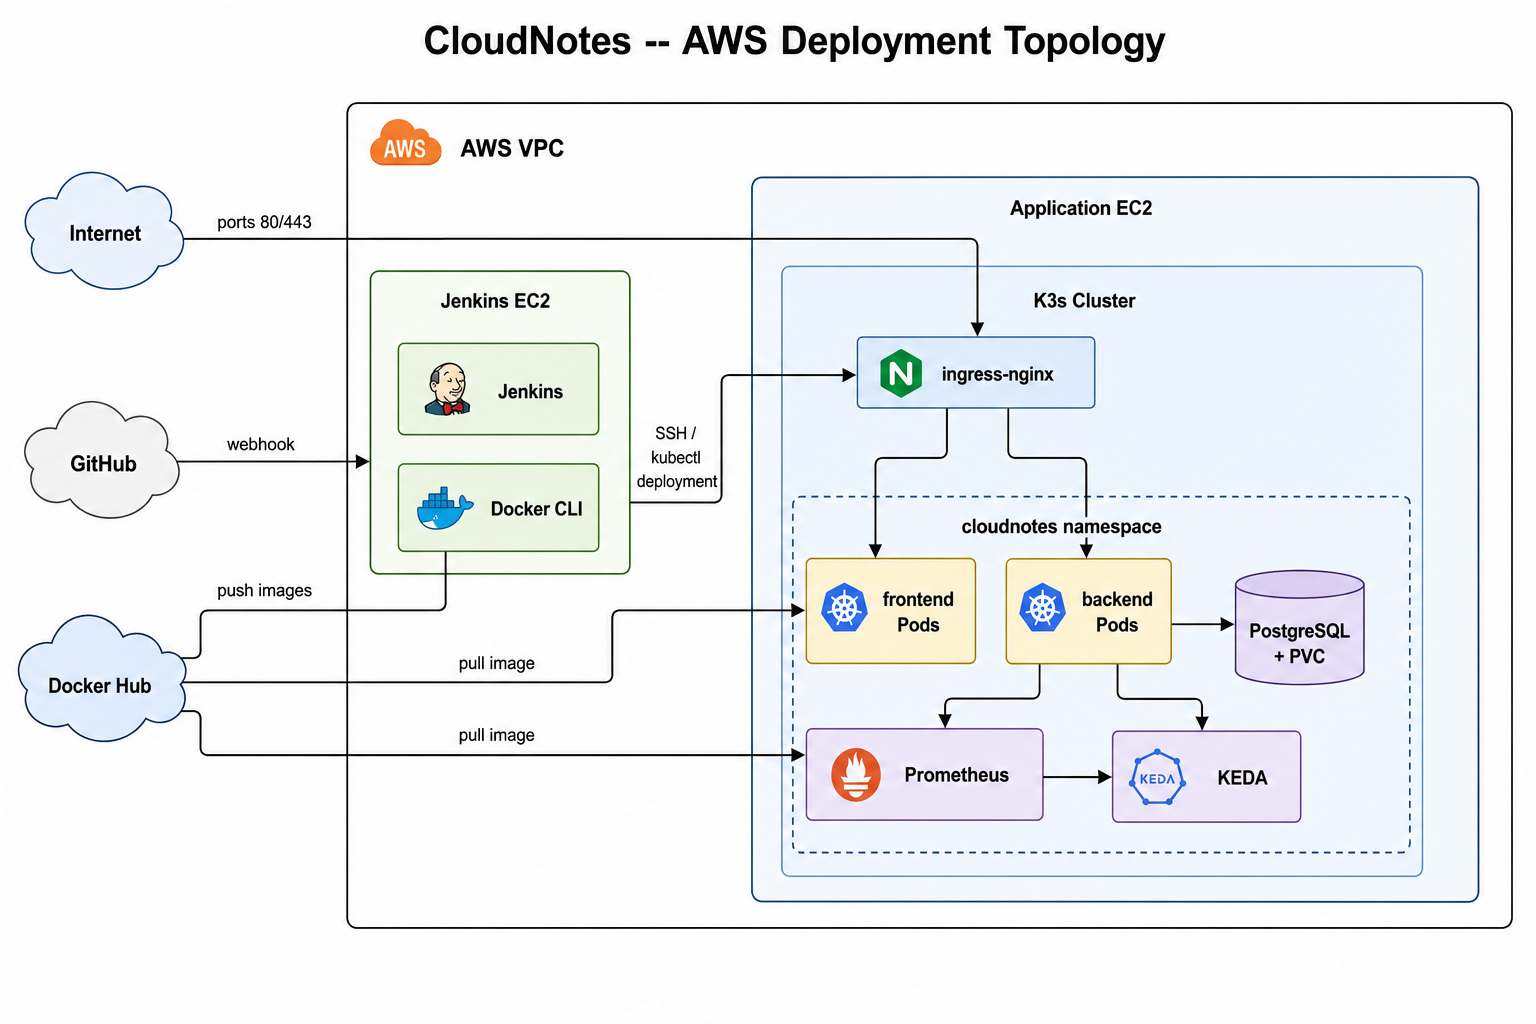
\includegraphics[width=0.82\linewidth,height=0.42\textheight,keepaspectratio]{deployment_topology.png}
\caption{AWS deployment topology and trust boundaries}
\label{fig:deployment_topology}
\end{figure}

\section{Traffic-Based Horizontal Scaling}
Kubernetes is used for orchestration and horizontal scaling; no Vertical Pod Autoscaler is configured. The frontend and backend Deployments start with two replicas to provide baseline availability. KEDA ScaledObjects define minimum and maximum replica counts of two to five for the backend and two to four for the frontend.

Prometheus scrapes the backend \texttt{/metrics} endpoint every 15 seconds. KEDA evaluates the PromQL expression shown in Equation~\ref{eq:rps}, where $R$ is the total API request rate. This is a direct traffic signal: more API requests result in a larger value of $R$ and therefore trigger additional replicas when the configured threshold is exceeded.

\begin{equation}
R = \sum \operatorname{rate}(\texttt{flask\_http\_request\_total}[1m])
\label{eq:rps}
\end{equation}

KEDA polls every 15 seconds and applies a cooldown period when demand falls. The frontend follows the API request-rate signal because browser interactions requiring application processing are routed through the API. Resource requests and limits support scheduling only; no component automatically increases a pod's CPU or memory allocation.

\section{Application Request Lifecycle}
For a create-note operation, ingress routes the API request to the backend, which validates and stores the note in PostgreSQL, increments \texttt{notes\_created\_total}, and returns JSON. Prometheus then collects the HTTP and business metrics for Grafana. The same pattern applies to updates and deletes. Figure~\ref{fig:note_sequence} presents this flow.

\begin{figure}[htbp]
\centering
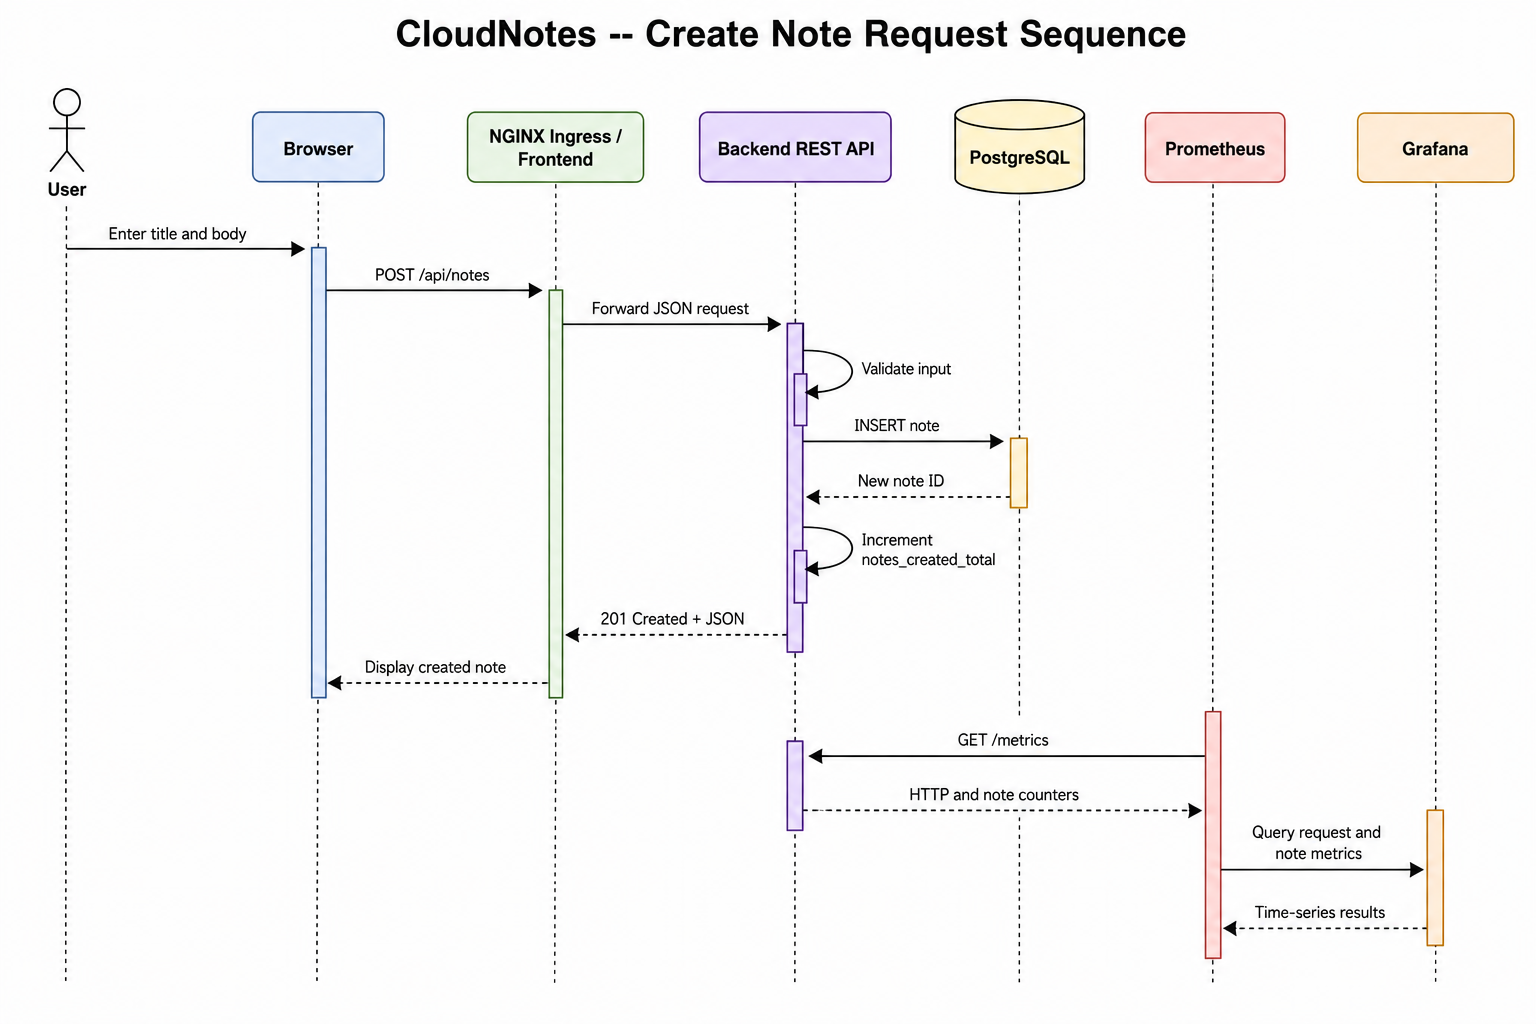
\includegraphics[width=0.82\linewidth,height=0.42\textheight,keepaspectratio]{create_note_sequence.png}
\caption{Sequence of a create-note request and metric collection}
\label{fig:note_sequence}
\end{figure}

\subsection{Data Model}
Each note has an identifier, title, body, and creation timestamp. Only the backend accesses PostgreSQL, preserving the frontend's API boundary. Figure~\ref{fig:data_model} shows the model.

\begin{figure}[htbp]
\centering
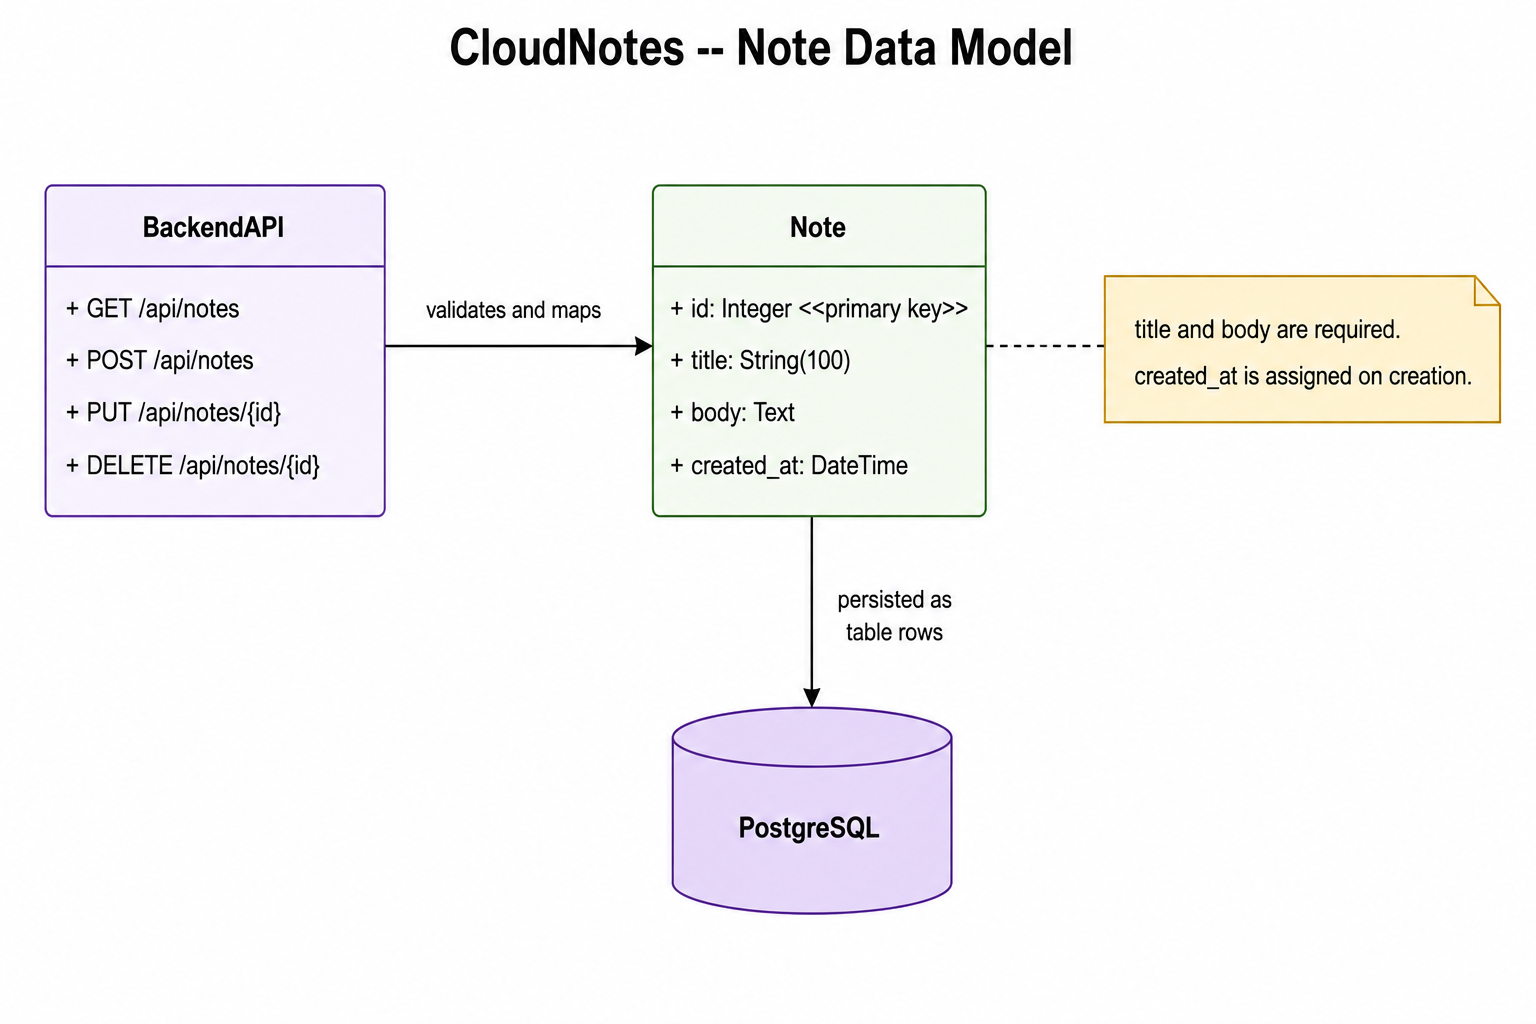
\includegraphics[width=0.82\linewidth,height=0.42\textheight,keepaspectratio]{note_data_model.png}
\caption{CloudNotes persistence model}
\label{fig:data_model}
\end{figure}

\section{CI/CD Pipeline}
GitHub push webhooks trigger Jenkins; GitHub Actions is not used. Jenkins checks out the source, tests the backend image, scans for secrets and image vulnerabilities, publishes build-number-tagged images to Docker Hub, and deploys them through SSH and \texttt{kubectl}. The deployment waits for rollout status and an ingress health check. A failure in any stage stops the release, while \texttt{disableConcurrentBuilds} prevents conflicting deployments. Figures~\ref{fig:pipeline_sequence} and \ref{fig:cicd_monitoring} show this flow.

\begin{figure}[htbp]
\centering
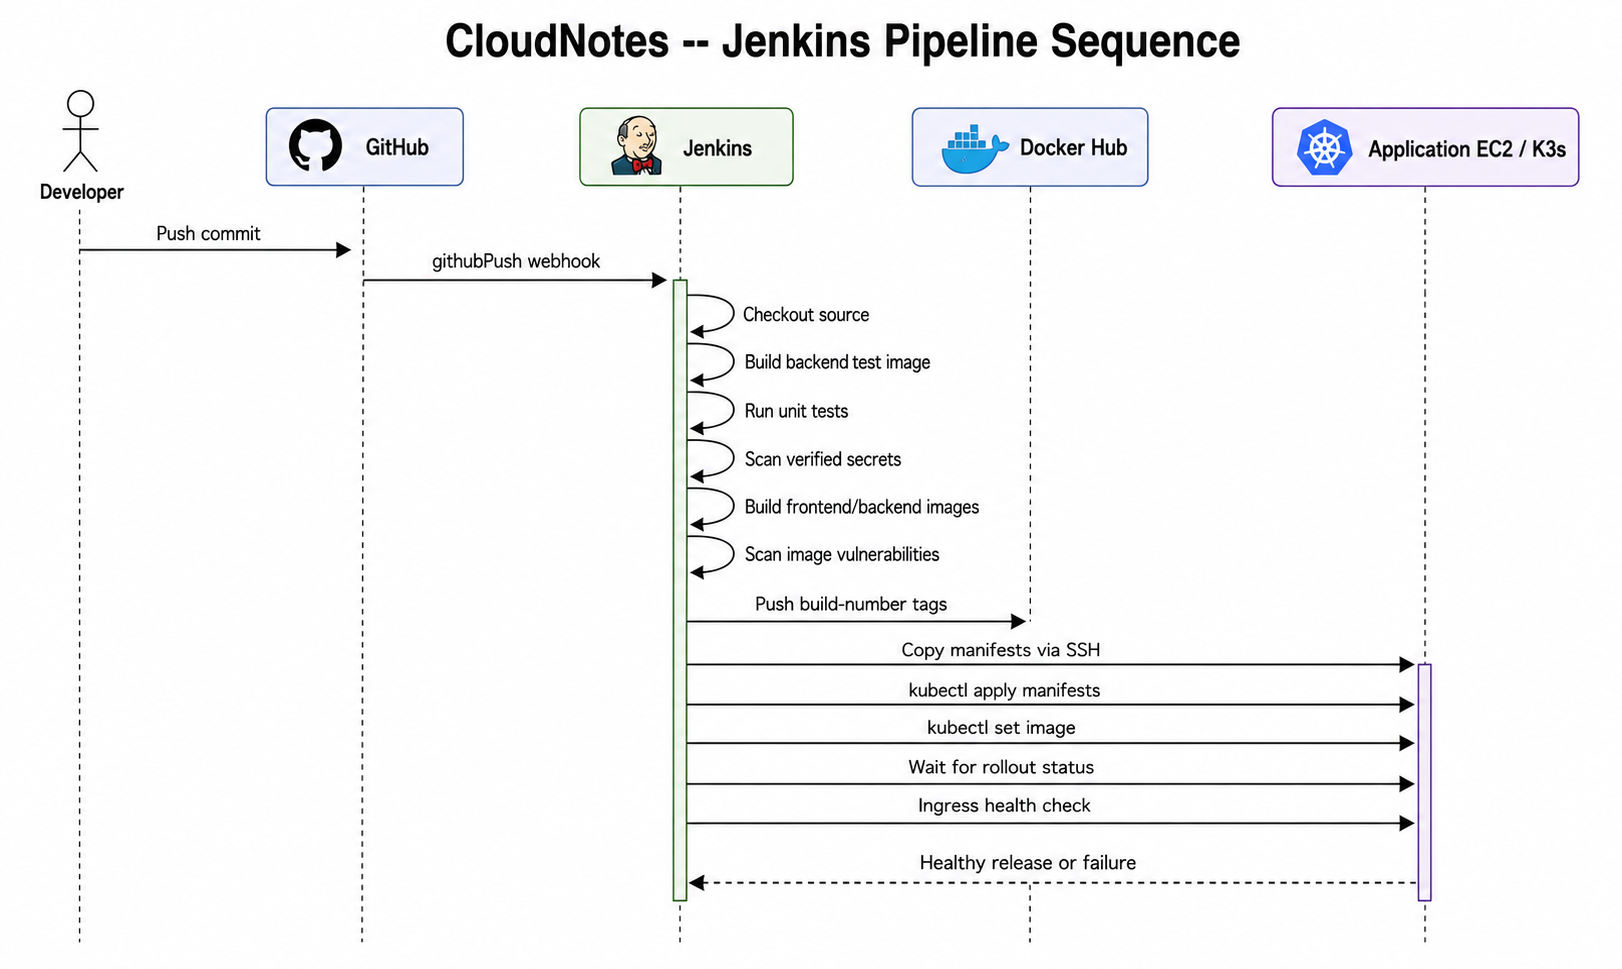
\includegraphics[width=0.82\linewidth,height=0.42\textheight,keepaspectratio]{pipeline_sequence.png}
\caption{Automated Jenkins pipeline sequence}
\label{fig:pipeline_sequence}
\end{figure}

\begin{figure}[htbp]
\centering
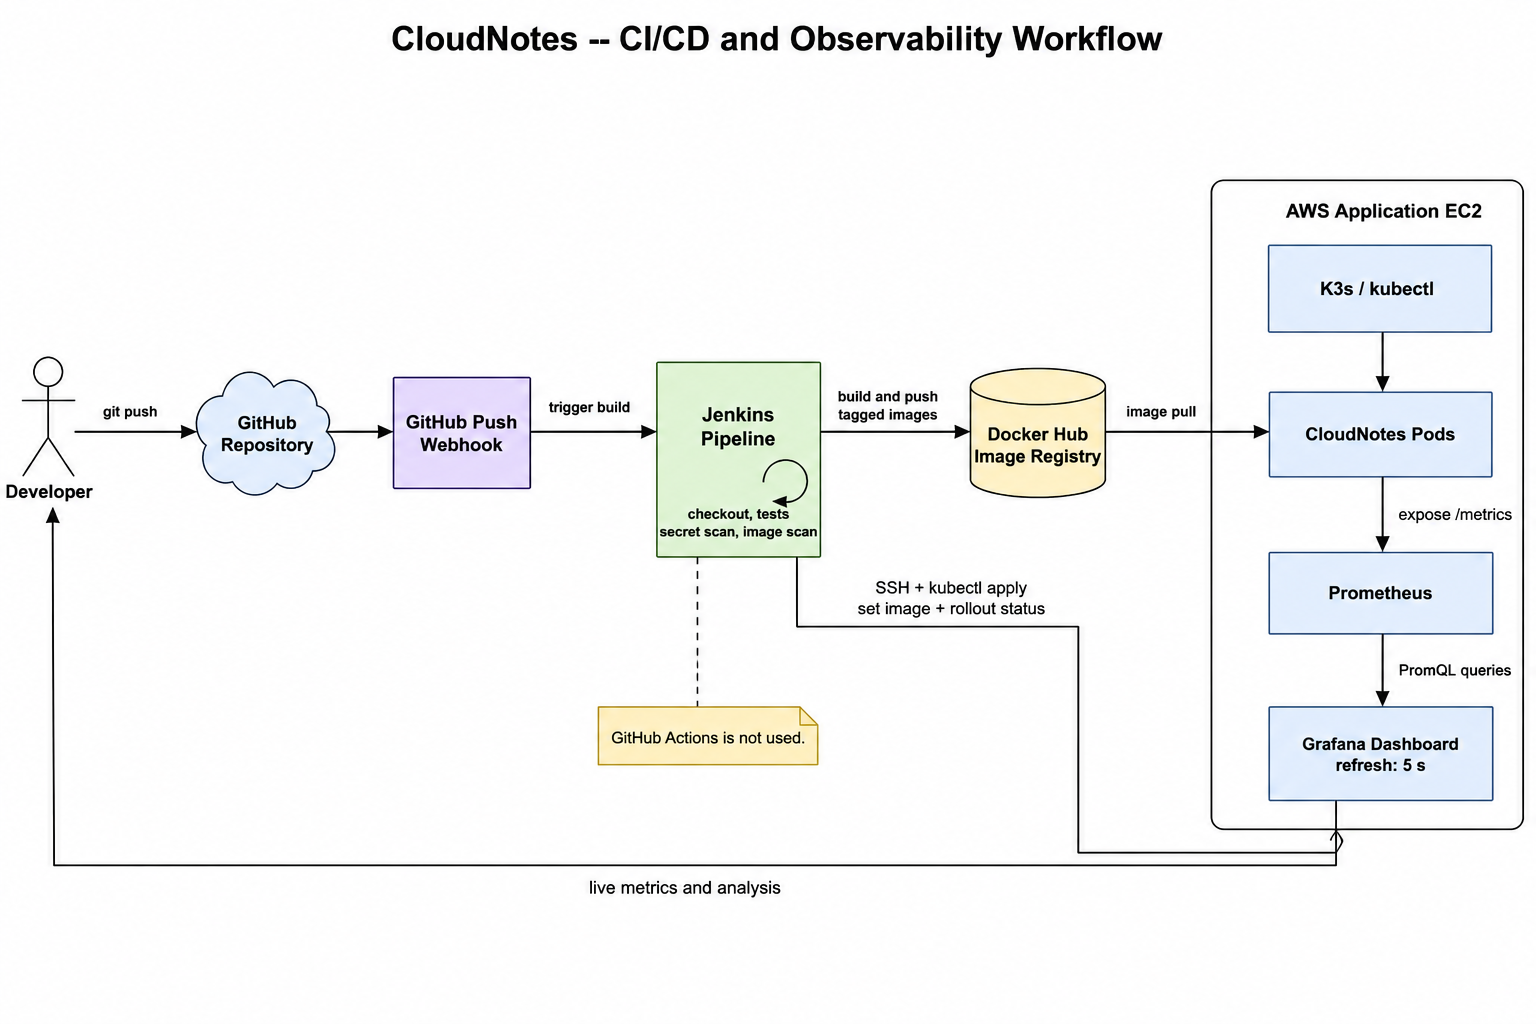
\includegraphics[width=0.82\linewidth,height=0.42\textheight,keepaspectratio]{cicd_observability_flow.png}
\caption{Jenkins CI/CD pipeline and observability workflow}
\label{fig:cicd_monitoring}
\end{figure}

\section{Monitoring and Live Dashboards}
Prometheus collects HTTP and note-operation metrics from the backend and evaluates availability, error-rate, latency, and activity alert rules in the local Compose configuration and Kubernetes Prometheus ConfigMap. Grafana provisions a local Compose dashboard with availability, note events, request rate, errors, latency, and memory panels. The Kubernetes manifests do not deploy Grafana. Alert rules define conditions; notification delivery requires an independently configured Alertmanager receiver. Figure~\ref{fig:observability_architecture} shows this feedback loop.

\begin{figure}[htbp]
\centering
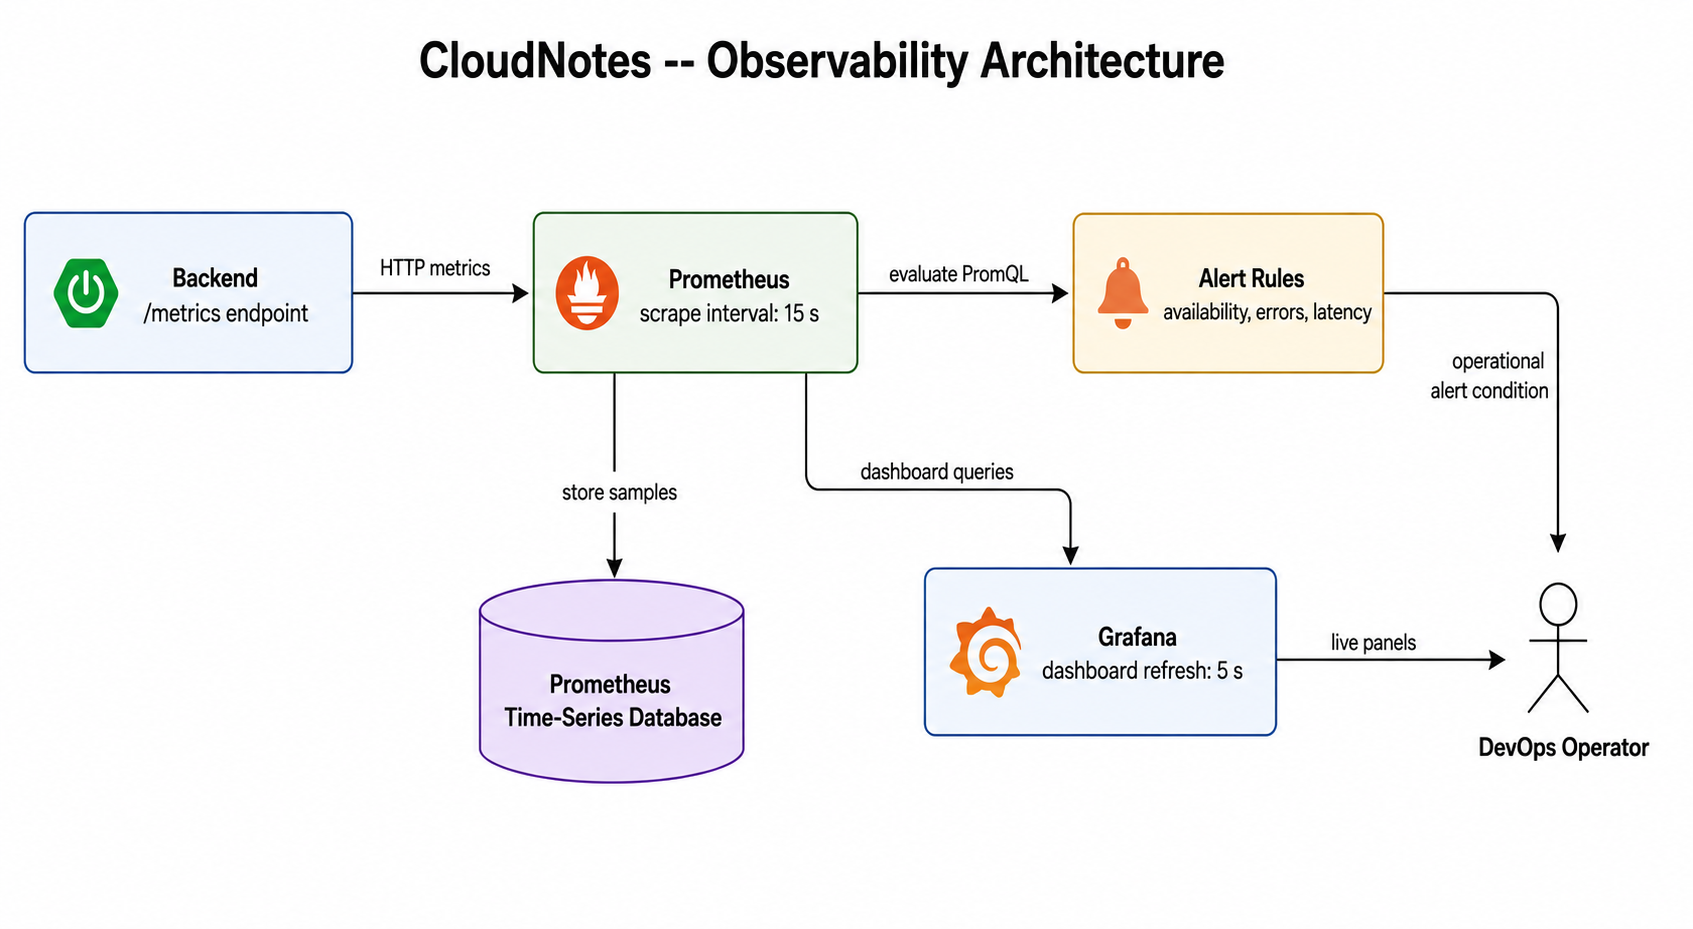
\includegraphics[width=0.82\linewidth,height=0.42\textheight,keepaspectratio]{observability_architecture.png}
\caption{Prometheus, alerting, and Grafana observability architecture}
\label{fig:observability_architecture}
\end{figure}

\section{Security, Reliability, and Validation Strategy}
Jenkins credentials protect Docker Hub and SSH access; PostgreSQL values are provided through a Kubernetes Secret and must be changed before public deployment. Secret and image scans, security groups, health probes, persistent storage, rollout checks, and Prometheus alerts provide the main security and reliability controls. Validation includes Terraform validation, backend tests, rollout/health checks, and a traffic test that verifies KEDA replica changes.

\section{Test Plan and Acceptance Criteria}
The test plan combines functional, infrastructure, delivery, scaling, and observability checks. A test is accepted only when its stated evidence is visible in the relevant tool output or application response. Table~\ref{tab:testplan} provides a concise acceptance plan suitable for a project demonstration.

\begin{table}[htbp]
\caption{Test plan and acceptance criteria}
\label{tab:testplan}
\centering
\begin{tabular}{p{0.21\textwidth}p{0.34\textwidth}p{0.33\textwidth}}
\hline
\textbf{Test area} & \textbf{Procedure} & \textbf{Acceptance evidence} \\
\hline
Note CRUD & Create, retrieve, search, update, and delete a note through the browser or API. & Correct JSON/UI response and persisted database state. \\
Container build & Build frontend and backend Docker images independently. & Successful image build and independently runnable service containers. \\
Terraform & Run formatting, initialization, validation, plan, and apply in an authorized AWS account. & Valid configuration and created EC2/S3 resources shown by Terraform output and AWS console. \\
Pipeline & Push a benign change to GitHub. & Jenkins webhook-triggered build executes tests, scans, image publication, rollout, and health check. \\
Scaling & Generate sustained API requests above the configured threshold. & Prometheus request rate rises; KEDA reports activity; Deployment replica count increases within allowed range. \\
Monitoring & Perform note operations and view Grafana. & Dashboard panels refresh with availability, request, note-event, latency, and error data. \\
Recovery & Delete a backend pod after deployment. & Kubernetes recreates the pod and readiness returns to healthy state. \\
\hline
\end{tabular}
\end{table}

\section{Risk Analysis and Mitigation}
Cloud deployments introduce technical and operational risks that must be considered even in an academic implementation. Credential exposure is mitigated through Jenkins credential bindings, non-interactive login, secret scanning, and deployment-time secrets. Image vulnerabilities are mitigated through the Trivy scan stage, although image updates remain necessary as new vulnerabilities are disclosed. Incorrect infrastructure changes are mitigated by Terraform review, validation, and plan output before applying changes.

Availability risks include application errors, database failure, configuration errors, and unusual traffic spikes. Health probes, Deployment self-healing, persistent database storage, minimum replicas, and monitoring alerts reduce these risks. The single-node K3s deployment remains a limitation: an EC2 instance outage can interrupt the service. A future multi-node cluster, managed database, automated backups, and multi-zone architecture would reduce this residual risk. Cost risk is addressed by the Terraform billing alarm, which sends an SNS notification when estimated AWS charges reach the configured threshold.

\section{Project Schedule}
Figure~\ref{fig:project_timeline} provides an evidence-based project timeline. The completed milestones use repository commit history: initial implementation began on 19 May 2026, CI/CD and monitoring hardening continued through 26 May 2026, and security/documentation refactoring concluded on 2 June 2026. Final validation, diagram preparation, and synopsis work are shown as planned work from 2 to 12 September 2026, so the document does not represent future work as completed.

\begin{figure}[htbp]
\centering
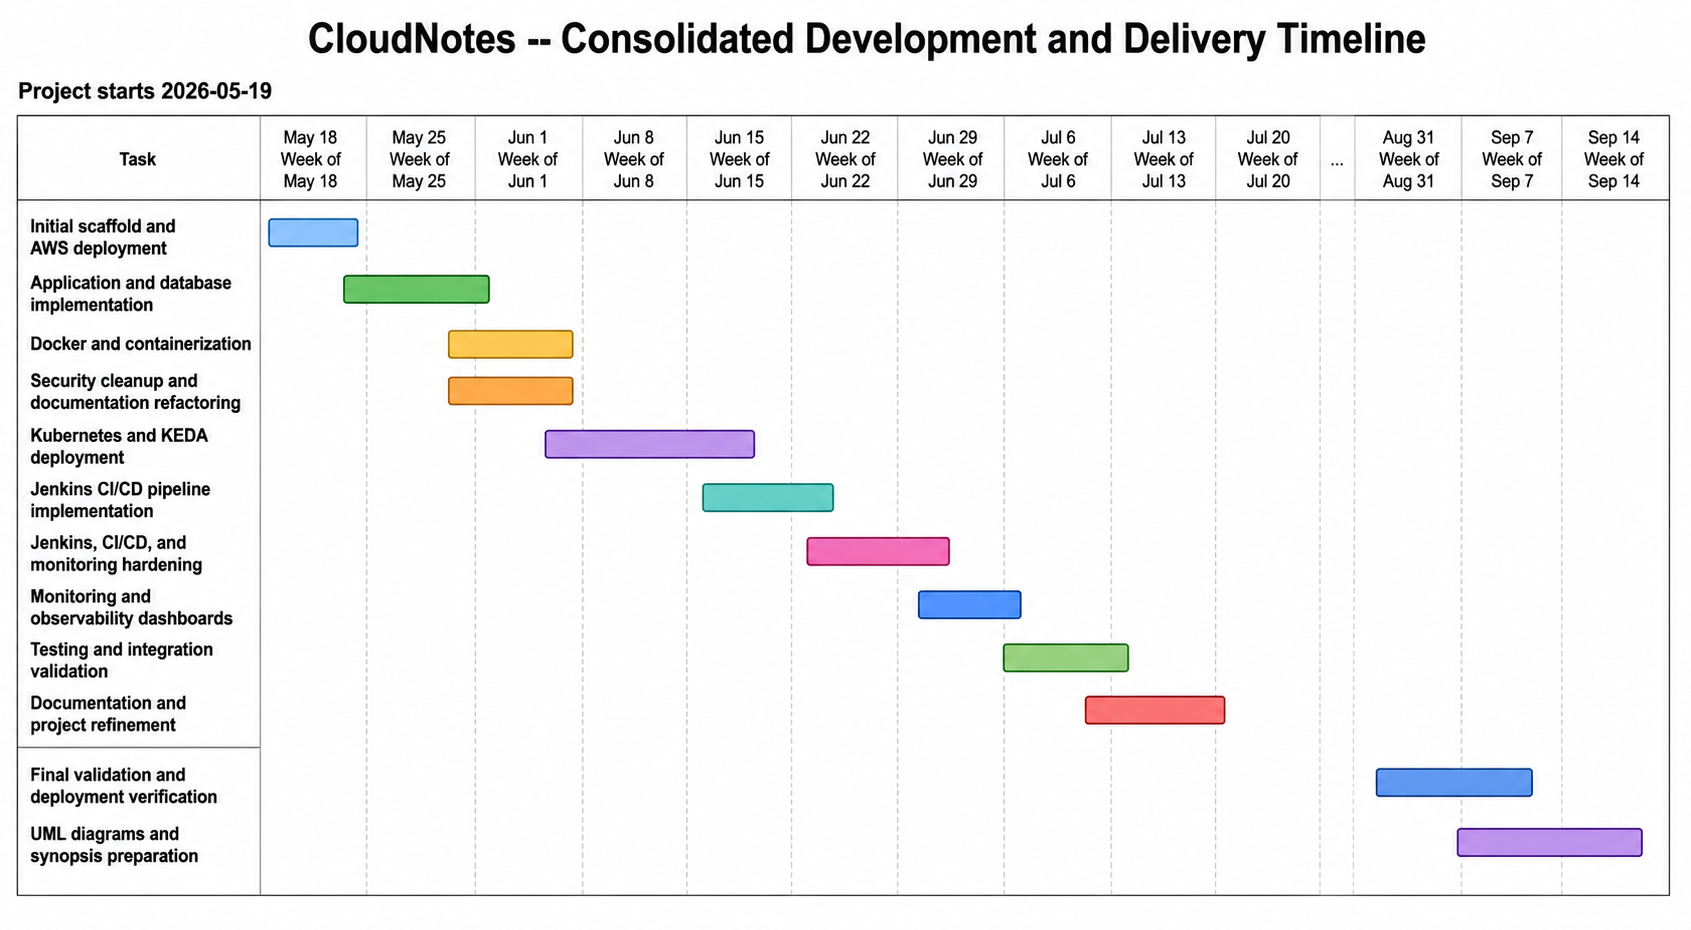
\includegraphics[width=0.82\linewidth,height=0.42\textheight,keepaspectratio]{project_timeline.png}
\caption{Illustrative CloudNotes development timeline}
\label{fig:project_timeline}
\end{figure}

\section{Requirements Traceability}
Table~\ref{tab:traceability} maps the specified DevOps requirements to their implementation artefacts.

\begin{table}[htbp]
\caption{Requirements traceability matrix}
\label{tab:traceability}
\centering
\begin{tabular}{p{0.25\textwidth}p{0.67\textwidth}}
\hline
\textbf{Requirement} & \textbf{Implementation evidence} \\
\hline
Docker images and independent services & Frontend and backend Dockerfiles, separate service directories, and Docker Compose configuration. \\
Kubernetes orchestration and horizontal scaling & Deployments, Services, Ingress, PersistentVolumeClaim, K3s, and KEDA ScaledObjects. \\
Traffic-based scaling; no vertical scaling & Prometheus request-rate PromQL triggers with defined minimum and maximum replicas; no Vertical Pod Autoscaler. \\
Terraform on AWS with EC2 and S3 & Terraform modules for VPC, EC2, and S3 resources using the AWS provider. \\
Prometheus metrics and analysis & Backend \texttt{/metrics} endpoint, scrape configuration, PromQL queries, and alert rules. \\
Grafana live dashboards & Provisioned Prometheus data source and dashboard with a five-second refresh interval. \\
GitHub, pipeline, webhooks; no GitHub Actions & GitHub repository webhook trigger and Jenkinsfile pipeline; no GitHub Actions workflow. \\
\hline
\end{tabular}
\end{table}

\section{Expected Outcomes and Future Enhancements}
The intended outcome is a repeatable demonstration environment in which a code push can trigger validation and delivery, application pods serve user traffic through Kubernetes, and replica counts can increase as request rate rises. A demonstration must capture current evidence of rollout, request-rate scaling, and live dashboards before claiming those runtime outcomes. Operators can use the configured Grafana dashboard and Prometheus alert conditions to inspect availability and performance.

Future work can add TLS certificates and a custom domain, replace placeholder secrets with a managed secret store, use a managed database service, add alert notifications, retain monitoring data on persistent storage, and introduce load testing to validate scaling thresholds. A multi-node Kubernetes cluster and multi-availability-zone deployment would further improve resilience.

\section{Conclusion}
CloudNotes combines containerization, AWS infrastructure as code, Kubernetes orchestration, traffic-based horizontal scaling, Jenkins CI/CD, and live observability in one coherent project. The architecture makes each application tier independently deployable, uses Terraform for repeatable AWS provisioning, and uses Prometheus metrics to inform KEDA scaling decisions. By using GitHub webhooks with Jenkins and by excluding GitHub Actions and vertical scaling, the project satisfies the stated DevOps constraints while providing a realistic foundation for future extension.

\begin{thebibliography}{00}
\bibitem{docker} Docker, ``Docker Documentation.'' [Online]. Available: \url{https://docs.docker.com/}
\bibitem{kubernetes} Kubernetes, ``Kubernetes Documentation.'' [Online]. Available: \url{https://kubernetes.io/docs/}
\bibitem{terraform} HashiCorp, ``Terraform AWS Provider Documentation.'' [Online]. Available: \url{https://registry.terraform.io/providers/hashicorp/aws/latest/docs}
\bibitem{keda} KEDA, ``KEDA Documentation.'' [Online]. Available: \url{https://keda.sh/docs/}
\bibitem{prometheus} Prometheus, ``Prometheus Documentation.'' [Online]. Available: \url{https://prometheus.io/docs/}
\bibitem{grafana} Grafana Labs, ``Grafana Documentation.'' [Online]. Available: \url{https://grafana.com/docs/grafana/}
\end{thebibliography}

\end{document}
